\section{Analytical results}

\subsection{Transfer orbit}

In this first part we only consider the gravitational pull from the Earth. We would like to calculate the speed needed for Webb to reach a distance \(r_1 = 1.5\) million km at the peak of the transfer orbit, starting from a lower distance \(r_0 = 6800\) km as shown in \autoref{fig:schema_transfert}. Let \(m\) be the mass of Webb, \(m_T\) the mass of the Earth, \(v_0\) and \(v_1\) the required start and end speed respectively. From conservation of TODO, we can write
\begin{equation}
    r_0 v_0 = r_1 v_1
    \label{eq:conservation_moment_inertie}
\end{equation}
and using conservation of energy
\begin{equation}
    \frac{1}{2} m v_0^2 - G \frac{m m_T}{r_0} = \frac{1}{2} m v_1^2 - G \frac{m m_T}{r_1}
    \label{eq:conservation_energy}
\end{equation}
where \(G = 6.674 \cdot 10{-11}\) \si{\meter\cubed\per\kilo\gram\per\second\squared}. Using \autoref{eq:conservation_moment_intertie} we get
\begin{equation}
    v_0 = \frac{r_1 v_1}{r_0}
    \label{eq:v0_substitution}
\end{equation}
which we can then substitute in \autoref{eq:conservation_energy} to get
\begin{equation}
    \frac{1}{2} m \left(\frac{r_1}{r_0}\right)^2 v_1^2 - G \frac{m m_T}{r_0} = \frac{1}{2} m v_1^2 - G \frac{m m_T}{r_1}
\end{equation}
Solving for \(v_1\) we get the following expression:
\begin{equation}
    v_1 = r_0 \sqrt{2 G m_T \frac{\frac{1}{r_0}-\frac{1}{r_1}}{r_1^2-r_0^2}}
\end{equation}
Using \autoref{eq:v0_substitution}, we have
\begin{equation}
    v_0 = r_1 \sqrt{2 G m_T \frac{\frac{1}{r_0}-\frac{1}{r_1}}{r_1^2-r_0^2}}
\end{equation}


\begin{figure}[h]
    \centering
    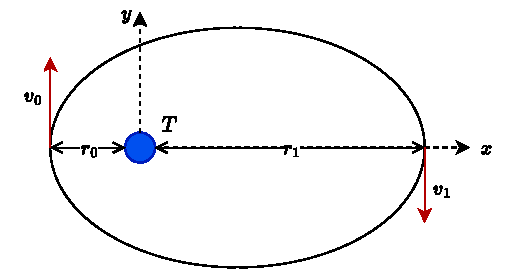
\includegraphics[width=0.6\linewidth]{figures/transfert.pdf}
    \caption{Schematic of the transfer orbit of Webb}
    \label{fig:schema_transfert}
\end{figure}

\begin{figure}[h]
    \centering
    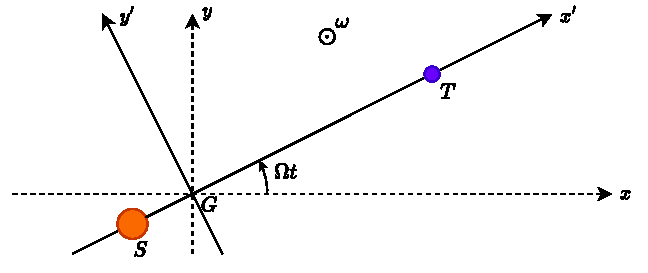
\includegraphics[width=0.8\linewidth]{figures/referentiel.pdf}
    \caption{Schematic of the transfer orbit of Webb}
    \label{fig:schema_referentiel}
\end{figure}

Mecanical energy (WRONG):
\begin{equation}
    E_\textrm{mec} = \frac{1}{2} m \left( v_x^2 + v_y^2 \right) - G \frac{m m_T}{r_T} - G \frac{m m_S}{r_S}
\end{equation}
